\section{Evaluation} \label{sec:evaluation}
We will now evaluate how our encoding scheme performs on tag width and memory usage for the applications of Software-Defined IXPs and service chaining.

\subsection{Service Chaining}
Recall that for the service chaining setting, attributes of an FEC are middleboxes that packets in the FEC must visit, and that these attributes are ordered.
To evaluate service chains, we simulate a network policy by generating a set of random middlebox paths. The number of attributes in the service chaining application is equal to the number of distinct types of middleboxes. Sherry et. al~\cite{Sherry:2012} gives a lower bound of 11 middlebox categories, so we evaluate up to $M = 40$ middleboxes to emulate a reasonably sized network. 

To generate random paths over these $M$ middleboxes, we first assume that all service chains follow a fixed underlying ordering. A random starting point in the ordering is chosen, and a path is constructed by making random jumps to middleboxes further down the ordering, stopping once the end of the ordering is reached.

Next, to simulate conflicting orderings, we post-process each random path to add ordering conflicts. For each pair of adjacent middleboxes in a path, we swap their positions with some probability $p_{err}$. We chose a value of $5\%$ for $p_{err}$, as we believe reordering of middleboxes to be rare. 

\begin{figure}[t!] 
\begin{minipage}{1\linewidth}
\begin{subfigure}[b]{0.96\linewidth}
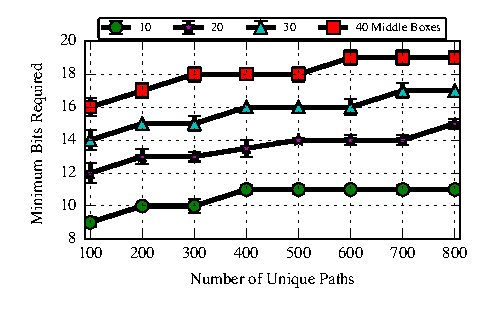
\includegraphics[width=\linewidth]{figures/service_chaining_minbits_ordered}
\end{subfigure} 
\end{minipage} 
\caption{Minimum number of bits required by our encoding scheme to encode every service chain as the number of service chains increases. The four lines represent the tag sizes required when encoding chains across 10, 20, 30, and 40 distinct middleboxes. All paths generated with a $5\%$ chance of reordering.}
\label{fig:chain_bits}
\end{figure}

Figure \ref{fig:chain_bits} evaluates the minimum widths required by our encoding scheme across varying numbers of random paths and middleboxes. Recall that if there are $N$ distinct paths, flat tagging requires $log_2(N)$ bits to encode every path. Since $log_2(800) = 9$, our encoding scheme requires roughly twice the tag width of flat tagging for this experiment. 

\begin{figure}[t!] 
\begin{minipage}{1\linewidth}
\begin{subfigure}[b]{0.96\linewidth}
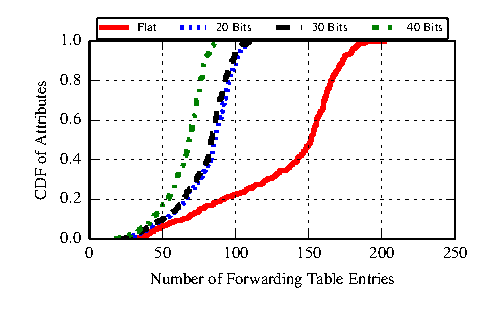
\includegraphics[width=\linewidth]{figures/attr_cdf}
\end{subfigure} 
\end{minipage} 
\caption{Minimum number of bits required by our encoding scheme to encode every service chain as the number of service chains increases. The four lines represent the tag sizes required when encoding chains across 10, 20, 30, and 40 distinct middleboxes. All paths generated with a $5\%$ chance of reordering.}
\label{fig:chain_rules}
\end{figure}

Figure \ref{fig:chain_rules} compares the number of rules required by our encoding scheme to the number of rules required by flat tags. Since our scheme uses less memory when the tag is permitted to be wider, we evaluate the memory usage for tag widths $[20,30,40]$. We observed that 20 bits was the minimum necessary for our tagging scheme on this dataset, as seen in Figure \ref{fig:chain_bits}, so we begin at that width. Flat tagging does not have any tuneable parameters for making a width-memory tradeoff, so it is only evaluated once.

The number of rules needed by our scheme is less than half that used by flat tagging in this application. While this is an improvement, we suspect the benefits will be much greater for real datasets, as there will be more redundancy in the paths for our encoding to exploit.


\subsection{Software-Defined IXPs}
To evaluate the Software-Defined IXP setting, we must identify what characteristics of an IXP determine tagging performance. For each packet in this setting, the attributes of a packet are the list of next-hop IXP participants which have announced routes to that packet's destination. Two packet share an FEC if they can take the same list of next-hops to exit the IXP fabric. An attribute (next-hop) is queried if there is some policy which wants to forward traffic to that next-hop. Therefore, to evaluate our scheme over Software-Defined IXPs, we need (1) route announcements and (2) forwarding policies. 


For route announcements, we used Routing Information dumps from the AMS-IX exchange point~\cite{ams-ix}, retrieved from the Routing Information Service raw data webpage~\cite{ris}. This dataset gave us access to 63 participants advertising over 600,000 prefixes. 
To simulate smaller instances when determining growth functions, we randomly sample subsets of all the IXP participants. We repeat this sampling procedure multiple times to average together multiple results.
To simulate interdomain forwarding policies, we generate a fixed number of forwarding actions that each forward to a random IXP participant. For our evaluations, only the participant that a policy forwards to is relevant, so we do not require a more detailed policy generation method. 

In the SDX and iSDX~\cite{sdx, isdx} solutions, tags are attached to the destination MAC field of packets, which has a limit of 48 bits. However, the iSDX solution attaches additional information to the MAC field, leaving only 37 bits available for tagging. Therefore, for our encoding scheme to be used in the iSDX system, our tags must fit within 37 bits. We use this limit when evaluating the number of rules required. 

Figure \ref{fig:bits} shows the number of bits required by our encoding scheme with uniformly randomly chosen IXP participant subsets, repeated 500 times for each subset size. In the worst case, 18 bits were required when considering all 63 participants. The graphs appear to show that the number of bits required scales linearly with the number of participants present in the active set. However, we believe that the number of bits required actually scales sublinearly with the size of the active set, and that the appearance of linear scaling is a consequence of our random sampling method. In order for the bits required to scale linearly, the number of attributes per FEC would have to also increase linearly in the size of the IXP, but we suspect this is not the case. Even if the number of bits required were indeed to scale linearly, extrapolating out the graph yields that, in the worst case, there could be over 100 attributes to encode, allowing very complex forwarding policies.

\begin{figure}[t!] 
\begin{minipage}{1\linewidth}
\begin{subfigure}[b]{0.96\linewidth}
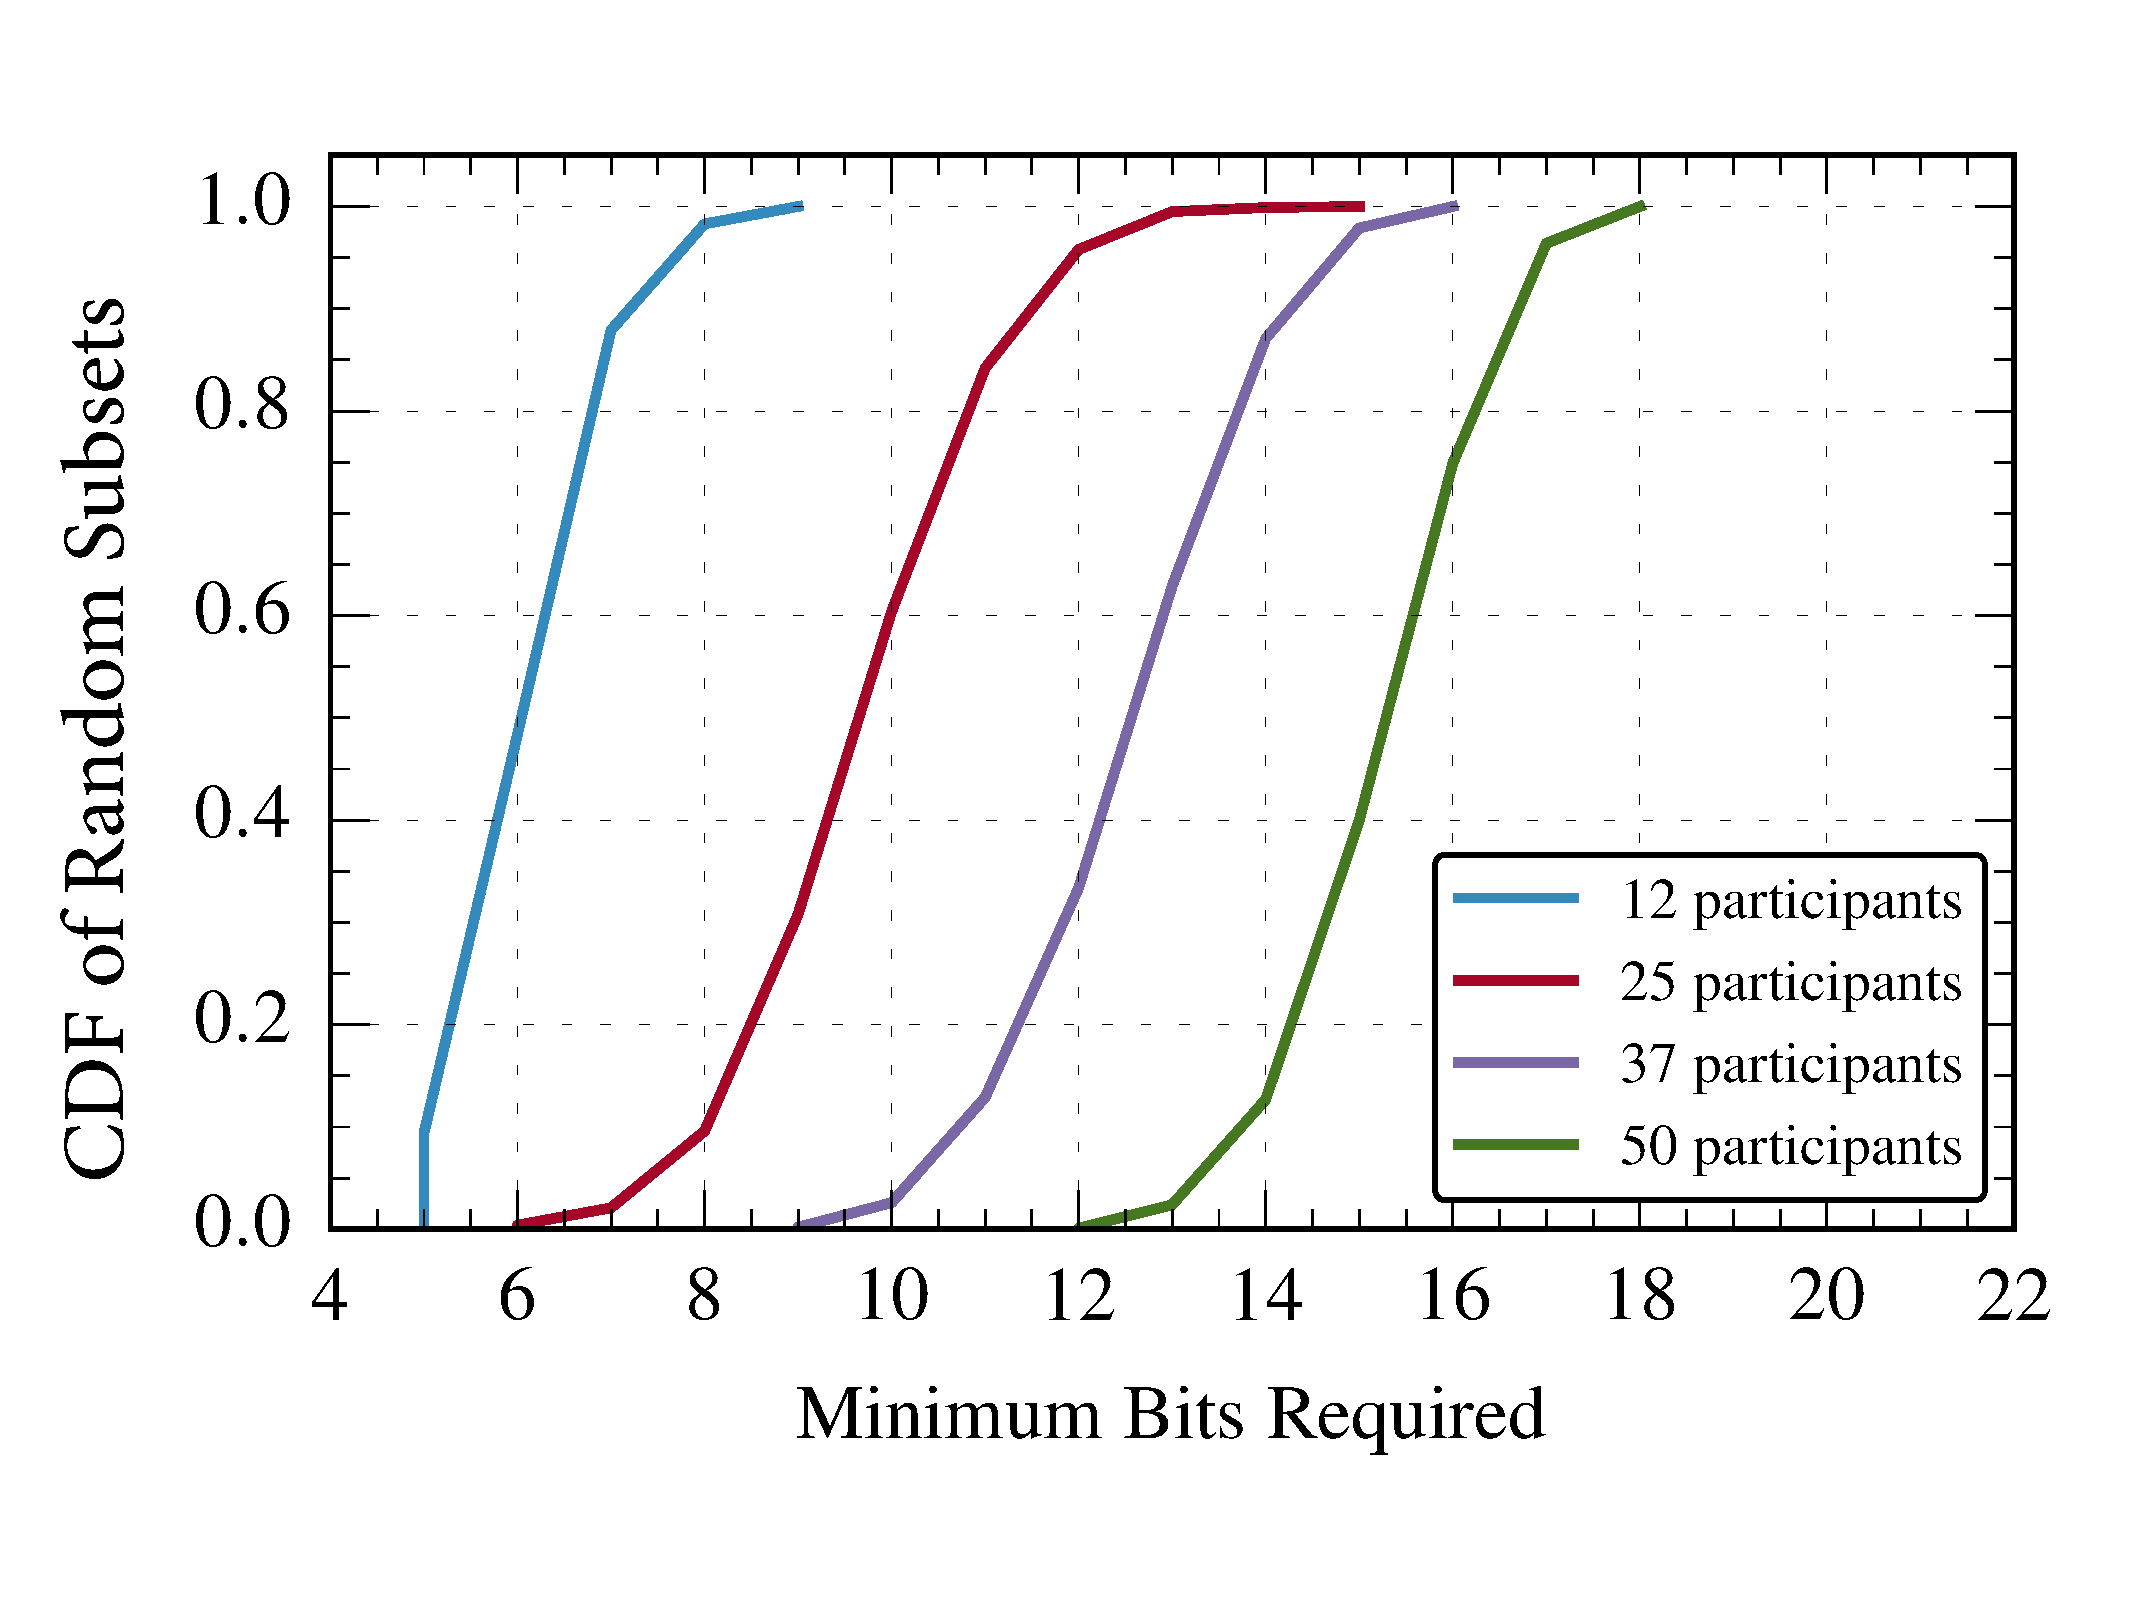
\includegraphics[width=\linewidth]{figures/bit_counts}
\end{subfigure} 
\end{minipage} 
\caption{Minimum number of bits required by a feasible solution for a random policy which forwards to a random subset of participants.}
\label{fig:bits}
\end{figure}


\begin{figure}[t!] 
\begin{minipage}{1\linewidth}
\begin{subfigure}[b]{0.96\linewidth}
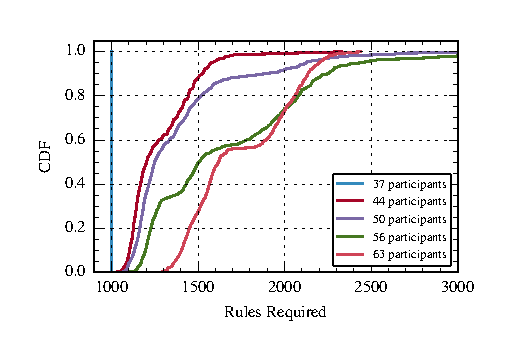
\includegraphics[width=\linewidth]{figures/rule_cdf}
\end{subfigure} 
\end{minipage} 
\caption{Number of rules required after encoding for a random policy of 1000 rules to random subsets of participants.}
\label{fig:rules}
\end{figure}

Figure \ref{fig:rules} shows the number of rules required by our encoding scheme after running the greedy algorithm up to the limit of 37 bits. In this experiment, we began with a baseline forwarding policy of 1000 rules, with each rule querying a random attribute.

forwarding to a participant chosen uniformly at random from a random active set. The experiment was repeated 500 times for each subset size, and the number of rules required after applying our encoding was plotted. When the active set is of size 37 or fewer, all participants can fit into a single mask, resulting in zero rule inflation. For active sets of size greater than 37, we can see that the inflation factor is at most 2 in the average case and 3 in the worst case for all active sets. 


\begin{figure}[t!] 
\begin{minipage}{1\linewidth}
\begin{subfigure}[b]{0.96\linewidth}
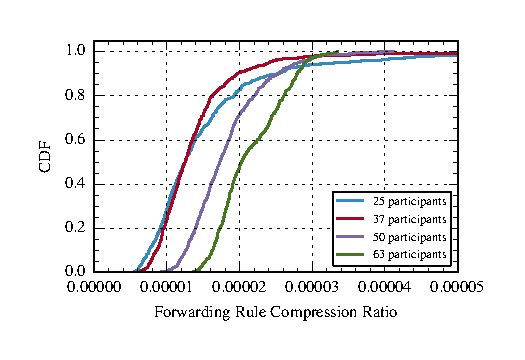
\includegraphics[width=\linewidth]{figures/compression_cdf}
\end{subfigure} 
\end{minipage} 
\caption{Ratio of flow rules required by our encoding algorithm versus the uncompressed
case on random policies involving random subsets of participants.}
\label{fig:compression}
\end{figure}

Figure \ref{fig:compression} shows how the number of flow rules generated by our approach compares to the naive case of zero compression. The compression ratio of our approach versus the naive approach is 20,000 to 1 in the worst case for all active set sizes, and 50,000 to 1 in the median case.


\begin{figure}[t!] 
\begin{minipage}{1\linewidth}
\begin{subfigure}[b]{0.96\linewidth}
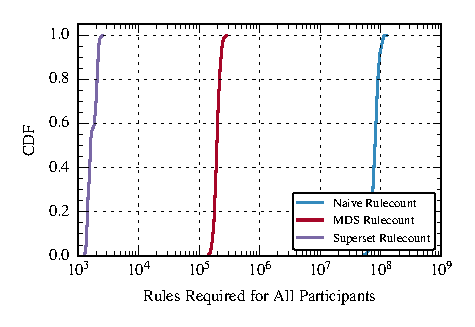
\includegraphics[width=\linewidth]{figures/comparison_cdf}
\end{subfigure} 
\end{minipage} 
\caption{Comparison of the number of flow rules required by our encoding algorithm to the previous state-of-the-art MDS encoding algorithm and the uncompressed case for a random policy involving all participants.}
\label{fig:comparison}
\end{figure}


Figure \ref{fig:comparison} compares our approach to the uncompressed case, as well as to the previous state-of-the-art, the MDS algorithm used in the original SDX system~\cite{sdx}. The comparisons were all made using the same approach of generating 1000 random rules, with the exception of the MDS simulation. The MDS algorithm requires each prefix's default next-hop as part of the input, so in each trial we chose next-hops uniformly at random from the list of available next-hops. The graph shows that our approach consistently compresses the number of flow rules by two orders of magnitude greater than the MDS algorithm, which itself compressed the number of flow rules required by the naive case by three orders of magnitude. 

